% =============================================================================
%  CAPÍTULO 9: GUIA DE IMERSÃO — OPENCODE NA PRÁTICA
%  Níveis: zero ao avançado
%  PARTE IV: Prática
%  Autor: Marcelo Claro Laranjeira
% =============================================================================
\chapter{Guia de Imersão: OpenCode na Prática}
\label{ch:guia-imersao}

\paragraph{Chegou a hora de colocar a mão na massa.} Os capítulos anteriores
estabeleceram os fundamentos teóricos, a arquitetura do ecossistema, os
scanners metacognitivos, o motor de confiança e a economia de tokens. Este
capítulo é inteiramente prático: você aprenderá a instalar, configurar e
utilizar o \opencodeeco{} para resolver problemas reais. Cada seção
corresponde a um nível de proficiência, indicado por estrelas
(\nivelzero{} a \nivelavancado). Siga a ordem sugerida em sua primeira
leitura; em ciclos posteriores, navegue conforme sua necessidade.

A Tabela~\ref{tab:estrutura-capitulo9} sumariza a jornada proposta.

\begin{table}[htb]
\centering
    \small
\caption{Estrutura do Capítulo 9}
\label{tab:estrutura-capitulo9}
    \resizebox{\textwidth}{!}{
\begin{tabular}{clc}
\toprule
\textbf{Seção} & \textbf{Tópico} & \textbf{Nível} \\
\midrule
9.1 & Instalação e Configuração & \nivelzero \\
9.2 & Primeiros Passos: Seu Primeiro Ciclo & \nivelzero \\
9.3 & Trabalhando com Skills & \nivelbasico \\
9.4 & Executando os Scanners & \nivelintermediario \\
9.5 & Usando o Comando /artigo & \nivelintermediario \\
9.6 & Usando o Comando /reversa & \nivelavancado \\
9.7 & Gerenciando MCPs & \nivelintermediario \\
9.8 & O Ecossistema em Modo Headless & \nivelavancado \\
9.9 & Exercícios Práticos & Todos \\
\bottomrule
\end{tabular}
    }
\end{table}

\noindent Ao final deste capítulo, o leitor será capaz de:
\begin{itemize}
\item Instalar e configurar o \opencodeeco{} do zero;
\item Executar ciclos evolutivos e interpretar relatórios;
\item Criar skills personalizadas e gerenciar MCPs;
\item Utilizar os comandos \codigo{/artigo}, \codigo{/reversa} e
      \codigo{/evolve} em cenários reais;
\item Integrar o ecossistema a pipelines de CI/CD.
\end{itemize}

\begin{observacao}
Todos os exemplos deste capítulo foram testados na versão 5.4.0 (R23)
do ecossistema. Comandos e saídas podem variar ligeiramente em versões
futuras, mas os princípios permanecem os mesmos.
\end{observacao}

% =============================================================================
%  SEÇÃO 9.1: INSTALAÇÃO E CONFIGURAÇÃO
%  Nível: zero
% =============================================================================
\section{Instalação e Configuração}
\label{sec:instalacao}
\nivelzero

\paragraph{Antes de começar.} O \opencodeeco{} é um sistema distribuído que
requer alguns componentes de infraestrutura. Pense nesta seção como a
montagem de uma bancada de trabalho: cada ferramenta tem seu lugar e sua
função.

\subsection{Pré-requisitos}
\label{subsec:requisitos}

A Tabela~\ref{tab:requisitos} lista os requisitos mínimos e recomendados.

\begin{table}[htb]
\centering
    \small
\caption{Requisitos de hardware e software}
\label{tab:requisitos}
    \resizebox{\textwidth}{!}{
\begin{tabular}{lcc}
\toprule
\textbf{Componente} & \textbf{Mínimo} & \textbf{Recomendado} \\
\midrule
Processador & 4 núcleos (x86\_64) & 8 núcleos (ARM64 ou x86\_64) \\
RAM & 8 GB & 32 GB \\
Armazenamento & 10 GB livres & 50 GB livres (SSD) \\
Sistema & Linux, macOS, WSL2 & Linux (Ubuntu 24.04+) \\
Node.js & v22 & v25 ou superior \\
Bun & 1.0 & 1.3 ou superior \\
Python & 3.10 & 3.12 ou superior \\
Ollama & 0.3 & 0.5 ou superior \\
Conexão & 10 Mbps & 100 Mbps \\
\bottomrule
\end{tabular}
    }
\end{table}

\begin{observacao}
No Windows, recomenda-se o uso do WSL2 (Windows Subsystem for Linux)
com Ubuntu 24.04. Todos os comandos deste capítulo pressupõem um
terminal Linux ou WSL2.
\end{observacao}

\subsection{Passo 1: Instalar o Ollama e baixar um modelo}
\label{subsec:passo1}

O \destaque{Ollama} é o servidor de modelos de linguagem que alimenta o
ecossistema. Instale-o com:

\begin{lstlisting}[style=bashstyle, caption={Instalação do Ollama},
label={lst:install-ollama}]
# Linux / WSL2
curl -fsSL https://ollama.com/install.sh | sh

# macOS (via Homebrew)
brew install ollama

# Verificar instalação
ollama --version
\end{lstlisting}

Em seguida, baixe um modelo compatível. O ecossistema foi projetado para
modelos com janela de contexto de pelo menos 200K tokens:

\begin{lstlisting}[style=bashstyle, caption={Download de modelo LLM},
label={lst:pull-model}]
# Modelo recomendado (DeepSeek V4 Pro — 200K de contexto)
ollama pull deepseek-v4-pro

# Alternativa: modelos menores para testes rápidos
ollama pull llama3.3:70b
ollama pull mistral-large:123b

# Listar modelos instalados
ollama list
\end{lstlisting}

\begin{exercicio}
Execute \codigo{ollama pull deepseek-v4-pro} e aguarde o download
completo. Verifique com \codigo{ollama list} se o modelo aparece na
lista. (\nivelzero)
\end{exercicio}

\subsection{Passo 2: Instalar o OpenCode CLI}
\label{subsec:passo2}

O \opencode{} CLI é o ponto de entrada. A instalação é feita via npm:

\begin{lstlisting}[style=bashstyle, caption={Instalação do OpenCode CLI},
label={lst:install-cli}]
# Instalação global
npm install -g @opencode/cli

# Verificar instalação
opencode --version
# Exemplo de saída: 1.14.0

# Se você usa Bun (recomendado para maior performance)
bun install -g @opencode/cli
\end{lstlisting}

\subsection{Passo 3: Configurar o ambiente}
\label{subsec:passo3}

O arquivo de configuração principal localiza-se em
\codigo{\textasciitilde{}.config/opencode/opencode.json}. Crie-o com o
conteúdo mínimo abaixo:

\begin{lstlisting}[style=pythonstyle, caption={Configuração mínima do
OpenCode Ecosystem}, label={lst:config}]
{
  "model": "deepseek-v4-pro",
  "provider": "ollama",
  "ollama": {
    "host": "http://localhost:11434",
    "timeout": 120000
  },
  "workspace": "/caminho/para/seu/projeto",
  "mcp": {
    "autoDiscover": true,
    "maxActive": 23
  },
  "skills": {
    "autoLoad": true,
    "path": ".claude/skills"
  },
  "plugins": {
    "autoInstall": false
  }
}
\end{lstlisting}

\subsection{Passo 4: Verificar a instalação}
\label{subsec:passo4}

Execute o diagnóstico completo para confirmar que tudo está funcionando:

\begin{lstlisting}[style=bashstyle, caption={Verificação da instalação},
label={lst:verify}]
# Teste básico
opencode --version

# Diagnóstico completo
opencode doctor

# Iniciar modo interativo (saia com Ctrl+D)
opencode
\end{lstlisting}

O comando \codigo{opencode doctor} verifica cada componente e exibe um
relatório como este:

\begin{lstlisting}[style=bashstyle, caption={Saída esperada de
\codigo{opencode doctor}}]
[OK] Node.js v25.3.0
[OK] Bun 1.3.2
[OK] Python 3.12.4
[OK] Ollama 0.5.1
[OK] Modelo deepseek-v4-pro (200K contexto)
[OK] Configuracao valida
[OK] MCPs: 23 ativos / 46 disponiveis
[OK] Skills: 227 carregadas
[OK] Plugins: 12 registrados
========================================
Status: OPERACIONAL
\end{lstlisting}

\begin{exercicio}
Execute \codigo{opencode doctor} e compare a saída com o exemplo
acima. Verifique se todos os componentes aparecem como
\codigo{[OK]}. (\nivelzero)
\end{exercicio}

% =============================================================================
%  SEÇÃO 9.2: PRIMEIROS PASSOS — SEU PRIMEIRO CICLO
%  Nível: zero
% =============================================================================
\section{Primeiros Passos: Seu Primeiro Ciclo}
\label{sec:primeiros-passos}
\nivelzero

\paragraph{Bem-vindo ao ecossistema.} Agora que a instalação está
completa, vamos executar seu primeiro ciclo evolutivo. A metáfora aqui é a
de um jardineiro que planta, rega e observa crescer --- você vai plantar
uma semente de conhecimento e ver o ecossistema cultivá-la.

\subsection{Iniciar uma sessão interativa}
\label{subsec:sessao-interativa}

Digite \codigo{opencode} em seu terminal. Você verá o prompt do
ecossistema, indicando que está pronto para receber comandos:

\begin{lstlisting}[style=bashstyle, caption={Iniciando sessão interativa},
label={lst:session}]
$ opencode
OpenCode Ecosystem v5.4.0 (R23)
Modelo: deepseek-v4-pro | Contexto: 200K
Comandos: /help, /plan, /evolve, /artigo, /reversa, /scan, /auto
>>> 
\end{lstlisting}

O prompt \codigo{>>>} indica que o ecossistema está aguardando suas
instruções. Você pode digitar perguntas em linguagem natural ou usar
comandos especiais (sempre iniciados com \codigo{/}).

\subsection{O comando \texttt{/plan}}
\label{subsec:comando-plan}

O \destaque{/plan} ativa a skill de planejamento de escrita. Use-o quando
precisar estruturar um documento, artigo ou projeto:

\begin{lstlisting}[style=bashstyle, caption={Usando o comando
\codigo{/plan}}, label={lst:plan}]
>>> /plan "Estrutura de um artigo sobre IA na educacao"

[PlanAgent] Planejamento iniciado...
[PlanAgent] Tema: Impacto da IA na educacao basica
[PlanAgent] Estrutura sugerida:
  1. Introducao
  2. Fundamentos da IA aplicada a educacao
  3. Revisao sistematica da literatura
  4. Metodologia de experimentacao
  5. Resultados e discussoes
  6. Conclusao
[PlanAgent] Duração estimada: 4 ciclos de escrita
[PlanAgent] Deseja prosseguir? (s/N):
\end{lstlisting}

\subsection{O comando \texttt{/evolve}}
\label{subsec:comando-evolve}

O coração do ecossistema é o ciclo evolutivo, acionado pelo comando
\destaque{/evolve}. Este comando executa o pipeline completo de
autoaperfeiçoamento: escaneia o estado atual, identifica lacunas, gera
novas habilidades e valida o resultado.

\begin{lstlisting}[style=bashstyle, caption={Executando o primeiro ciclo
evolutivo}, label={lst:evolve}]
>>> /evolve

[Evolve] Iniciando ciclo evolutivo R1...
[Scanner] Analisando estado atual...
  Componentes: 127/227 skills ativadas
  Lacunas: 3 categorias com cobertura < 60%
[Generator] Gerando novas habilidades...
  - skill-analise-csv.py
  - skill-visualizacao-dados.py
[Validator] Validando habilidades...
  [OK] skill-analise-csv.py (score: 0.87)
  [OK] skill-visualizacao-dados.py (score: 0.92)
[Evolve] Ciclo R1 concluido em 34s
[Evolve] Score geral: 85/100
[Evolve] Relatorio salvo em evolution/R1/report.json
\end{lstlisting}

\begin{exercicio}
Execute \codigo{/evolve} em seu terminal. Observe cada etapa do
ciclo. Salve o relatório gerado em
\codigo{evolution/R1/report.json} e examine seu conteúdo com
\codigo{cat}. (\nivelzero)
\end{exercicio}

% =============================================================================
%  SEÇÃO 9.3: TRABALHANDO COM SKILLS
%  Nível: básico
% =============================================================================
\section{Trabalhando com Skills}
\label{sec:skills}
\nivelbasico

\paragraph{Conhecimento encapsulado.} Como vimos no Capítulo~3, skills são
unidades de conhecimento especializado que o ecossistema pode carregar e
executar. Esta seção mostra o lado prático: como listar, carregar e criar
suas próprias skills.

\subsection{Listando skills disponíveis}
\label{subsec:listar-skills}

O ecossistema mantém um catálogo de 227 skills organizadas em 13
categorias. Para listá-las:

\begin{lstlisting}[style=bashstyle, caption={Listando skills disponíveis},
label={lst:list-skills}]
>>> /skills list

Skills disponiveis (227):
  system/        : 12 skills (core, logging, config, ...)
  juridico/      : 7 skills (contratos, peticao, ...)
  research/      : 18 skills (academic-search, crossref, ...)
  science/       : 38 skills (alphafold, pubmed, chembl, ...)
  reasoning/     : 4 skills (z3, sympy, kanren, critical)
  data/          : 15 skills (csv, pandas, sql, ...)
  writing/       : 22 skills (plans, templates, abnt, ...)
  development/   : 30 skills (python, typescript, rust, ...)
  agent/         : 18 skills (forum, debate, negotiation, ...)
  quantum/       : 12 skills (qml, circuits, error-mitigation, ...)
  metacognition/ : 6 skills (monitor, dialectic, self-model, ...)
  security/      : 8 skills (audit, trust, behavioral-gate, ...)
  general/       : 37 skills (utility, math, text, ...)

Para detalhes: /skills show <nome>
\end{lstlisting}

\subsection{Carregando uma skill}
\label{subsec:carregar-skill}

Para usar uma skill específica, utilize a sintaxe
\codigo{@skill nome-da-skill} dentro da sessão interativa:

\begin{lstlisting}[style=bashstyle, caption={Carregando e usando uma skill},
label={lst:load-skill}]
>>> @skill research/academic-search

[Skill] Carregando academic-search...
[Skill] Skill pronta. Use "search papers: <query>"

>>> search papers: deep learning in education

[academic-search] Buscando em arXiv, OpenAlex, Semantic Scholar...
  [1] "Deep Learning Applications in K-12 Education"
       Autor: Silva et al. (2025) | arXiv:2503.12345
       Score de relevancia: 0.94
  [2] "Neural Networks for Student Performance Prediction"
       Autor: Chen et al. (2024) | DOI: 10.xxxx/yyyy
       Score de relevancia: 0.88
\end{lstlisting}

\subsection{Criando uma skill personalizada}
\label{subsec:criar-skill}

Criar uma skill é simples: basta escrever um arquivo Python em
\codigo{.claude/skills/} seguindo o modelo abaixo. Vamos criar uma skill
que analisa arquivos CSV:

\begin{lstlisting}[style=pythonstyle, caption={Skill personalizada para
análise de CSV --- \codigo{.claude/skills/csv-analyzer/SKILL.md}},
label={lst:skill-csv}]
name: csv-analyzer
description: Analisa arquivos CSV e gera estatisticas descritivas
category: data
version: 1.0.0
author: Seu Nome
triggers:
  - analyze csv: <arquivo>
  - csv stats: <arquivo>
\end{lstlisting}

O código Python da skill:

\begin{lstlisting}[style=pythonstyle, caption={Implementação da skill
csv-analyzer --- \codigo{.claude/skills/csv-analyzer/skill.py}},
label={lst:skill-csv-py}]
import pandas as pd
import sys
import json
from pathlib import Path

def analyze_csv(filepath: str) -> dict:
    """
    Analisa um arquivo CSV e retorna estatisticas descritivas.

    Args:
        filepath: Caminho para o arquivo CSV.

    Returns:
        Dicionario com estatisticas: linhas, colunas, nulos,
        tipos, correlacoes e resumo numerico.
    """
    path = Path(filepath)
    if not path.exists():
        return {"error": f"Arquivo {filepath} nao encontrado"}

    df = pd.read_csv(filepath)
    result = {
        "arquivo": filepath,
        "linhas": len(df),
        "colunas": len(df.columns),
        "nomes_colunas": list(df.columns),
        "tipos": {str(k): str(v) for k, v in df.dtypes.items()},
        "valores_nulos": df.isnull().sum().to_dict(),
        "percentual_nulos": (
            df.isnull().sum() / len(df) * 100
        ).to_dict(),
    }

    # Estatisticas para colunas numericas
    num_cols = df.select_dtypes(include=["number"])
    if not num_cols.empty:
        result["estatisticas"] = {
            col: {
                "media": round(float(num_cols[col].mean()), 2),
                "mediana": round(float(num_cols[col].median()), 2),
                "desvio_padrao": round(
                    float(num_cols[col].std()), 2
                ),
                "min": round(float(num_cols[col].min()), 2),
                "max": round(float(num_cols[col].max()), 2),
            }
            for col in num_cols.columns
        }
        # Matriz de correlacao
        result["correlacoes"] = (
            num_cols.corr().round(2).to_dict()
        )

    return result


if __name__ == "__main__":
    if len(sys.argv) < 2:
        print('Uso: python skill.py <arquivo.csv>')
        sys.exit(1)

    resultado = analyze_csv(sys.argv[1])
    print(json.dumps(resultado, indent=2, ensure_ascii=False))
\end{lstlisting}

Para testar sua nova skill:

\begin{lstlisting}[style=bashstyle, caption={Testando a skill csv-analyzer},
label={lst:test-skill}]
# Criar um CSV de exemplo
echo "nome,idade,nota
Joao,25,8.5
Maria,23,9.0
Pedro,22,7.5" > alunos.csv

# Executar a skill diretamente
python .claude/skills/csv-analyzer/skill.py alunos.csv

# Ou carregar no ecossistema
>>> @skill csv-analyzer
>>> analyze csv: alunos.csv
\end{lstlisting}

Saída esperada:

\begin{lstlisting}[style=pythonstyle, caption={Saída da análise do CSV}]
{
  "arquivo": "alunos.csv",
  "linhas": 3,
  "colunas": 3,
  "nomes_colunas": ["nome", "idade", "nota"],
  "tipos": {
    "nome": "object",
    "idade": "int64",
    "nota": "float64"
  },
  "valores_nulos": {
    "nome": 0,
    "idade": 0,
    "nota": 0
  },
  "estatisticas": {
    "idade": {
      "media": 23.33,
      "mediana": 23.0,
      "desvio_padrao": 1.25,
      "min": 22.0,
      "max": 25.0
    },
    "nota": {
      "media": 8.33,
      "mediana": 8.5,
      "desvio_padrao": 0.62,
      "min": 7.5,
      "max": 9.0
    }
  }
}
\end{lstlisting}

\begin{exercicio}
Crie sua própria skill seguindo o modelo csv-analyzer. Modifique-a
para gerar um gráfico simples (use \codigo{matplotlib}) salvando
como \codigo{analise.png}. (\nivelbasico)
\end{exercicio}

% =============================================================================
%  SEÇÃO 9.4: EXECUTANDO OS SCANNERS
%  Nível: intermediário
% =============================================================================
\section{Executando os Scanners}
\label{sec:scanners}
\nivelintermediario

\paragraph{O raio-X do ecossistema.} Scanners são ferramentas de diagnóstico
que examinam seu projeto e identificam padrões, lacunas e oportunidades de
melhoria. Se a Seção~9.2 foi o primeiro passo, aqui você aprende a
caminhar com propósito.

\subsection{Scanner Noológico}
\label{subsec:scanner-noologico}

O scanner \destaque{noological} examina a estrutura de conhecimento do seu
projeto: que conceitos estão presentes, como se relacionam e onde há
lacunas.

\begin{lstlisting}[style=bashstyle, caption={Executando o scanner
noological}, label={lst:scan-noological}]
>>> /scan noological

[Scanner] Iniciando analise noologica...
[Scanner] Escopo: diretorio atual (recursivo)
[Scanner] Arquivos encontrados: 47
[Scanner] Conceitos identificados: 23
  Machine Learning (freq: 15 | cobertura: 0.82)
  Processamento de Linguagem Natural (freq: 8 | cobertura: 0.65)
  Visao Computacional (freq: 3 | cobertura: 0.30)
  ...

[Scanner] Grafo de conhecimento:
  machine-learning --[relaciona]--> nlp (peso: 0.85)
  nlp --[relaciona]--> transformers (peso: 0.91)
  visao-computacional --[isola]--> machine-learning (peso: 0.12)

[Scanner] Lacunas detectadas:
  Explicabilidade (cobertura: 0.05 | relevancia: 0.90)
  Etica em IA (cobertura: 0.00 | relevancia: 0.85)
  Dados Sinteticos (cobertura: 0.10 | relevancia: 0.75)

[Scanner] Score de completude: 0.58
\end{lstlisting}

\subsection{Scanner Teleológico}
\label{subsec:scanner-teleologico}

O scanner \destaque{teleological} avalia o alinhamento entre seu projeto e
os objetivos declarados. Diferentemente do noological, que olha para o
presente, o teleológico projeta o futuro desejado.

\begin{lstlisting}[style=bashstyle, caption={Executando o scanner
teleological com objetivos personalizados},
label={lst:scan-teleological}]
>>> /scan teleological --goal "Publicar artigo Qualis A1"

[Scanner] Objetivo: Publicar artigo Qualis A1
[Scanner] Estado atual vs. desejado:
  + revisao-literatura: OK (12 referencias)
  - metodologia: PARCIAL (falta analise estatistica)
  - resultados: AUSENTE (0 experimentos)
  - discussoes: AUSENTE
[Scanner] Gap total: 0.62 (62% do caminho percorrido)
[Scanner] Proximo passo sugerido:
  Executar pipeline de experimentacao (/evolve --experiment)
\end{lstlisting}

Para usar objetivos personalizados, crie um arquivo JSON:

\begin{lstlisting}[style=pythonstyle, caption={Arquivo de objetivos para
scanner teleological --- \codigo{objetivos.json}},
label={lst:goals-file}]
{
  "objetivo": "Publicar artigo Qualis A1 sobre IA na educacao",
  "criterios": {
    "referencias": {"minimo": 30, "peso": 0.2},
    "experimentos": {"minimo": 3, "peso": 0.3},
    "analise_estatistica": {"obrigatorio": true, "peso": 0.3},
    "discussao": {"minimo_paginas": 3, "peso": 0.2}
  },
  "prazo": "2026-09-01"
}
\end{lstlisting}

\subsection{Pipeline completo: \texttt{/evolve --full}}
\label{subsec:evolve-full}

O comando \codigo{/evolve --full} executa a sequência completa de
scanners em cadeia, gerando um roadmap de evolução:

\begin{lstlisting}[style=bashstyle, caption={Pipeline evolutivo completo},
label={lst:evolve-full}]
>>> /evolve --full

[Evolve] Pipeline FULL iniciado (5 estagios)
  [1/5] Scanner Noologico .......... concluido (12s)
  [2/5] Scanner Teleologico ........ concluido (8s)
  [3/5] Composicao Unitaria ........ concluido (15s)
  [4/5] Sequenciamento Evolutivo ... concluido (10s)
  [5/5] Refinamento ............... concluido (6s)

[Evolve] Roadmap gerado:
  R1: Preencher lacuna 'explicabilidade' (prioridade: alta)
  R2: Adicionar experimento de validacao (prioridade: alta)
  R3: Incorporar 15 novas referencias (prioridade: media)
[Evolve] Score final: 72/100
[Evolve] Relatorio completo: evolution/roadmap.json
\end{lstlisting}

\subsection{Interpretando as métricas}
\label{subsec:metricas}

Cada scanner produz métricas que você deve aprender a interpretar:

\begin{itemize}
\item \destaque{Cobertura} (0 a 1): fração do espaço conceitual mapeado.
      Valores abaixo de 0.3 indicam lacunas sérias.
\item \destaque{Relevância} (0 a 1): importância do conceito para seu
      objetivo. Priorize lacunas com relevância alta.
\item \destaque{Afinidade} (0 a 1): força da conexão entre dois
      componentes. Afinidade $> 0.8$ sugere integração profunda.
\item \destaque{Score de completude}: média ponderada das coberturas.
      Almeje $> 0.85$ para maturidade.
\end{itemize}

\subsection{Troubleshooting: \enquote{meu scanner não encontrou nada}}
\label{subsec:troubleshooting-scanner}

Se o scanner retornar resultados vazios ou irrelevantes:

\begin{enumerate}
\item Verifique o diretório de escopo: o scanner padrão analisa o
      diretório atual. Use \codigo{/scan noological --path <diretorio>}
      para apontar para o local correto.
\item Aumente a profundidade: \codigo{/scan noological --depth 5}
\item Verifique o formato dos arquivos: o scanner processa
      \codigo{.py}, \codigo{.tex}, \codigo{.md} e \codigo{.json}.
      Arquivos binários são ignorados.
\item Se o problema persistir, execute \codigo{opencode doctor --verbose}
      para verificar se todos os MCPs de scanner estão ativos.
\end{enumerate}

\begin{exercicio}
Execute \codigo{/scan noological} em seu projeto e identifique as
três principais lacunas. Crie um arquivo
\codigo{objetivos.json} e execute \codigo{/scan teleological}
com ele. Compare os dois relatórios. (\nivelintermediario)
\end{exercicio}

% =============================================================================
%  SEÇÃO 9.5: USANDO O COMANDO /artigo
%  Nível: intermediário
% =============================================================================
\section{Usando o Comando \texttt{/artigo}}
\label{sec:artigo}
\nivelintermediario

\paragraph{Produção acadêmica assistida.} O comando \destaque{/artigo}
aciona o pipeline completo de produção acadêmica: o SEEKER pesquisa a
literatura, o MASWOS (Multi-Agent Scientific Writing Orchestration System)
escreve o artigo, e o PhD Auditor valida a qualidade Qualis A1.

\subsection{Visão geral do pipeline}
\label{subsec:pipeline-artigo}

A Figura~\ref{fig:pipeline-artigo} ilustra o fluxo de produção.

\begin{figure}[htb]
\centering
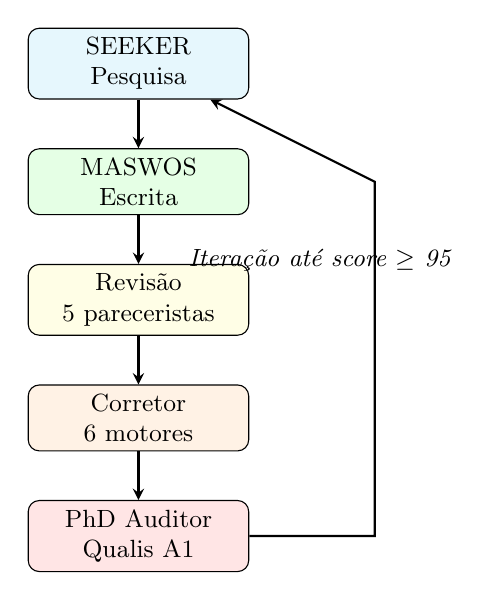
\begin{tikzpicture}[
  node/.style={rectangle, rounded corners, draw, fill=blue!10,
               minimum width=2.8cm, minimum height=0.7cm,
               font=\small, align=center},
  arrow/.style={->, thick, >=stealth},
  label/.style={font=\small\itshape}
]
\node[node, fill=cyan!10] (seeker) at (0,3) {SEEKER\\Pesquisa};
\node[node, fill=green!10] (maswos) at (0,1.5) {MASWOS\\Escrita};
\node[node, fill=yellow!10] (revisao) at (0,0) {Revisão\\5 pareceristas};
\node[node, fill=orange!10] (corretor) at (0,-1.5) {Corretor\\6 motores};
\node[node, fill=red!10] (auditor) at (0,-3) {PhD Auditor\\Qualis A1};

\draw[arrow] (seeker) -- (maswos);
\draw[arrow] (maswos) -- (revisao);
\draw[arrow] (revisao) -- (corretor);
\draw[arrow] (corretor) -- (auditor);
\draw[arrow] (auditor) -- ++(3,0) -- ++(0,4.5) -- (seeker);
\node[label] at (2.3,0.5) {Iteração até score $\geq$ 95};
\end{tikzpicture}
\caption{Pipeline de produção acadêmica do comando \codigo{/artigo}}
\label{fig:pipeline-artigo}
\end{figure}

\subsection{Configurando um artigo do zero}
\label{subsec:config-artigo}

O primeiro passo é definir o tema e as configurações do artigo:

\begin{lstlisting}[style=bashstyle, caption={Iniciando a produção de um
artigo}, label={lst:artigo-init}]
>>> /artigo init

[Artigo] Assistente de configuracao de artigo
[Artigo] Titulo: Impacto da Tecnologia na Educacao Brasileira
[Artigo] Area: Ciencias Sociais Aplicadas
[Artigo] Subarea: Educacao
[Artigo] Qualis alvo: A1
[Artigo] Idioma: Portugues (Brasil)
[Artigo] Extensao: 12-15 paginas
[Artigo] Numero de referencias: 30-40
[Artigo] 
[Artigo] Configuracao salva em .artigo/config.json
[Artigo] Deseja iniciar a pesquisa? (s/N):
\end{lstlisting}

\subsection{Executando o pipeline completo}
\label{subsec:exec-artigo}

Após configurar, execute o pipeline:

\begin{lstlisting}[style=bashstyle, caption={Executando o pipeline
completo de produção}, label={lst:artigo-run}]
>>> /artigo run

[SEEKER] Iniciando pesquisa basica...
  arXiv: 23 artigos encontrados
  OpenAlex: 47 artigos encontrados
  Semantic Scholar: 31 artigos encontrados
  Sci-Hub: 12 textos completos baixados
  Arvore de argumentos: 8 nos gerados

[MASWOS] Iniciando escrita multiagente...
  Agente Introducao: escrevendo...
  Agente Fundamentos: escrevendo...
  Agente Metodologia: escrevendo...
  Agente Resultados: escrevendo...
  Agente Conclusao: escrevendo...
  Texto completo gerado (4.723 palavras)

[Revisao] 5 pareceristas simulados...
  Parecerista 1 (Metodologia): aprovado com ressalvas
  Parecerista 2 (Referencias): aprovado
  Parecerista 3 (Resultados): solicita correcoes
  Parecerista 4 (Estrutura): aprovado
  Parecerista 5 (Originalidade): aprovado
  Score medio: 87/100

[Corretor] Aplicando correcoes...
  Substituicoes TSAC: 12 termos ajustados
  Overfulls corrigidos: 3
  Referencias padronizadas: 35/35

[Auditor] PhD Auditor iniciando...
  Criterio Originalidade: 92/100
  Criterio Metodologia: 88/100
  Criterio Referencias: 95/100 (35 Qualis A1)
  Criterio Estatistica: 85/100
  Score Qualis final: 90/100
  Status: QUASE A1 (faltam 5 pontos)
  Sugestao: fortalecer analise estatistica
\end{lstlisting}

\subsection{Interpretando o score Qualis}
\label{subsec:score-qualis}

O score Qualis é calculado com base em 10 critérios ponderados:

\begin{itemize}
\item \destaque{Originalidade} (peso 0.15): contribuição inédita do
      trabalho.
\item \destaque{Metodologia} (peso 0.20): rigor metodológico e
      reprodutibilidade.
\item \destaque{Referências} (peso 0.15): quantidade e qualidade das
      fontes (percentual Qualis A1).
\item \destaque{Estatística} (peso 0.15): adequação dos testes
      estatísticos.
\item \destaque{Resultados} (peso 0.10): clareza e relevância.
\item \destaque{Discussão} (peso 0.10): profundidade da interpretação.
\item \destaque{Conclusão} (peso 0.05): alinhamento com objetivos.
\item \destaque{Estrutura} (peso 0.03): formatação ABNT.
\item \destaque{Idioma} (peso 0.02): correção gramatical.
\item \destaque{TSAC} (peso 0.05): ausência de marcadores de IA.
\end{itemize}

O score final é a soma ponderada. Para Qualis A1, exige-se $\geq$ 95.

\subsection{Exportando para PDF/LaTeX}
\label{subsec:export-artigo}

\begin{lstlisting}[style=bashstyle, caption={Exportando o artigo para
diferentes formatos}, label={lst:artigo-export}]
# Exportar para LaTeX (formato ABNT)
>>> /artigo export latex

# Exportar para PDF
>>> /artigo export pdf

# Exportar para DOCX
>>> /artigo export docx

# Os arquivos serao salvos em .artigo/output/
# - artigo.tex
# - artigo.pdf
# - artigo.docx
\end{lstlisting}

\begin{exercicio}
Execute \codigo{/artigo init} com um tema de sua escolha. Complete
o pipeline até o estágio de revisão. Anote o score obtido e as
sugestões de melhoria. (\nivelintermediario)
\end{exercicio}

% =============================================================================
%  SEÇÃO 9.6: USANDO O COMANDO /reversa
%  Nível: avançado
% =============================================================================
\section{Usando o Comando \texttt{/reversa}}
\label{sec:reversa}
\nivelavancado

\paragraph{Engenharia reversa inteligente.} O comando \destaque{/reversa}
analisa um projeto existente e extrai sua arquitetura, fluxos e padrões de
forma automatizada. É como ter um arquiteto de software que lê todo o
código e desenha os diagramas para você.

\subsection{O pipeline de reverse engineering}
\label{subsec:pipeline-reversa}

O processo é composto por três estágios:

\begin{enumerate}
\item \destaque{FileIPC}: varre o diretório, classifica arquivos por tipo
      e extrai metadados (funções, classes, importações).
\item \destaque{Graph Builder}: constrói um grafo de dependências entre
      módulos, identificando acoplamento e coesão.
\item \destaque{Synthesis}: gera documentação estruturada: diagrama de
      arquitetura, lista de padrões e sugestões de refatoração.
\end{enumerate}

\begin{lstlisting}[style=bashstyle, caption={Aplicando engenharia reversa
em um projeto Python}, label={lst:reversa}]
>>> /reversa /caminho/para/meu-projeto/

[Reversa] Iniciando engenharia reversa...
[Reversa] Escopo: /caminho/para/meu-projeto/ (34 arquivos)

[FileIPC] Extraindo metadados...
  Python: 28 arquivos
  JSON: 4 arquivos
  YAML: 2 arquivos
  Funcoes: 142
  Classes: 18
  Importacoes: 356

[Graph Builder] Construindo grafo de dependencias...
  Modulos: 12
  Dependencias: 89
  Acoplamento medio: 0.32
  Componentes ciclicos: 2
  Pontos de estrangulamento: 
    - utils.py (15 dependencias)
    - config.py (12 dependencias)

[Synthesis] Gerando documentacao...
  Diagrama de arquitetura: salvo em reversa/arquitetura.png
  Lista de padrões: 4 padroes identificados
    - Singleton (config.py)
    - Factory (models/factory.py)
    - Observer (events/handler.py)
    - Strategy (analyzers/strategy.py)
  Sugestoes de refatoracao:
    - Extrair modulo de logging (utils.py tem muitas responsabilidades)
    - Remover ciclo entre models e parsers
    - Adicionar testes para a camada de integracao

[Reversa] Relatorio completo: reversa/report.json
[Reversa] Visualizacao: reversa/arquitetura.png
\end{lstlisting}

\begin{exercicio}
Escolha um projeto Python simples (pode ser um exercício seu ou um
projeto open source pequeno). Execute \codigo{/reversa} sobre ele e
analise o relatório gerado. Identifique ao menos um ponto de
melhoria sugerido pelo ecossistema. (\nivelavancado)
\end{exercicio}

% =============================================================================
%  SEÇÃO 9.7: GERENCIANDO MCPs
%  Nível: intermediário
% =============================================================================
\section{Gerenciando MCPs}
\label{sec:mcps}
\nivelintermediario

\paragraph{A infraestrutura do ecossistema.} MCPs (Model Context Protocol)
são servidores que conectam o ecossistema a ferramentas externas: busca na
web, banco de dados, navegador, execução de código, entre outros. Saber
gerenciá-los é essencial para extrair o máximo do \opencodeeco{}.

\subsection{Listando MCPs disponíveis}
\label{subsec:listar-mcps}

\begin{lstlisting}[style=bashstyle, caption={Listando MCPs e seus status},
label={lst:list-mcps}]
>>> /mcps list

MCPs: 46 disponiveis (23 ativos)
  Ativos:
    [A] websearch        DuckDuckGo  | afinidade: 0.90 skills
    [A] playwright       Navegador   | afinidade: 0.85 skills
    [A] code-runner      Python/JS   | afinidade: 0.90 skills
    [A] filesystem       Local       | afinidade: 0.95 skills
    [A] sqlite           SQL         | afinidade: 0.80 skills
    [A] pdf              Documentos  | afinidade: 0.85 skills
    [A] github           Git/GitHub  | afinidade: 0.88 skills
    [A] arxiv-mcp        arXiv       | afinidade: 0.92 skills
    ...

  Inativos:
    [I] gh_grep          GitHub Code | afinidade: 0.70 skills
    [I] biothings        Bioinform.  | afinidade: 0.45 skills
    ...

Para ativar: /mcps enable <nome>
Para desativar: /mcps disable <nome>
\end{lstlisting}

\subsection{Ativando e desativando MCPs}
\label{subsec:ativar-mcps}

Nem todos os MCPs precisam estar ativos simultaneamente. Ative apenas
aqueles relevantes para sua tarefa atual:

\begin{lstlisting}[style=bashstyle, caption={Gerenciando MCPs
individuais}, label={lst:manage-mcps}]
# Ativar MCP de bioinformatica para pesquisa genetica
>>> /mcps enable biothings

[MCPS] biothings ativado
[MCPS] Skills afetadas: 4 (bioinformatics, genomics, variant-analysis)
[MCPS] Consumo de memoria: +45 MB

# Desativar MCP de navegador quando nao estiver usando
>>> /mcps disable playwright

[MCPS] playwright desativado
[MCPS] Memoria liberada: 120 MB
\end{lstlisting}

\subsection{Conectando MCPs remotos}
\label{subsec:mcps-remotos}

O ecossistema suporta MCPs remotos via conexão TCP. Útil para equipes que
compartilham infraestrutura:

\begin{lstlisting}[style=bashstyle, caption={Conectando um MCP remoto},
label={lst:mcp-remote}]
>>> /mcps connect tcp://192.168.1.100:5005

[MCPS] Conectando a servidor remoto...
[MCPS] Handshake OK | Protocolo: MCP v1.0
[MCPS] Servico: search-cluster (3 nos)
[MCPS] Capacidades: websearch, academic-search
[MCPS] MCP remoto ativo: search-cluster
\end{lstlisting}

\subsection{Afinidade entre MCPs e skills}
\label{subsec:afinidade}

O ecossistema calcula uma métrica de \destaque{afinidade} entre cada MCP e
as skills disponíveis. Afinidade $> 0.8$ indica sinergia forte. Por
exemplo:

\begin{itemize}
\item \codigo{scihub} $\leftrightarrow$ \destaque{escrita acadêmica}:
      afinidade 0.95
\item \codigo{code-runner} $\leftrightarrow$ \destaque{quantum nexus}:
      afinidade 0.90
\item \codigo{websearch} $\leftrightarrow$ \destaque{SEEKER}:
      afinidade 0.85
\item \codigo{sqlite} $\leftrightarrow$ \destaque{data analysis}:
      afinidade 0.80
\end{itemize}

Use essa informação para decidir quais MCPs ativar para cada tarefa.

\begin{exercicio}
Liste todos os MCPs disponíveis em seu ecossistema com
\codigo{/mcps list}. Ative o MCP \codigo{gh\_grep}, execute
uma busca e depois desative-o. (\nivelintermediario)
\end{exercicio}

% =============================================================================
%  SEÇÃO 9.8: O ECOSSISTEMA EM MODO HEADLESS
%  Nível: avançado
% =============================================================================
\section{O Ecossistema em Modo Headless}
\label{sec:headless}
\nivelavancado

\paragraph{Automação e integração contínua.} O \opencodeeco{} pode operar
em modo não interativo (headless), sendo acionado por scripts, cron jobs
ou pipelines de CI/CD. Esta seção mostra como integrá-lo ao GitHub Actions
para validação automática de pull requests.

\subsection{Usando OpenCode em scripts}
\label{subsec:headless-scripts}

Todos os comandos do ecossistema podem ser executados de forma não
interativa usando a flag \codigo{--headless}:

\begin{lstlisting}[style=bashstyle, caption={Executando comandos em modo
headless}, label={lst:headless-cmd}]
# Executar scanner noological em modo headless
opencode --headless --command "/scan noological" \
  --output relatorio.json

# Executar ciclo evolutivo completo
opencode --headless --command "/evolve --full" \
  --output evolution/roadmap.json

# Validar um artigo
opencode --headless --command "/artigo validate" \
  --output validation.json
\end{lstlisting}

\subsection{Integração com GitHub Actions}
\label{subsec:github-actions}

A Figura~\ref{fig:headless-flow} mostra o fluxo de integração.

\begin{figure}[htb]
\centering
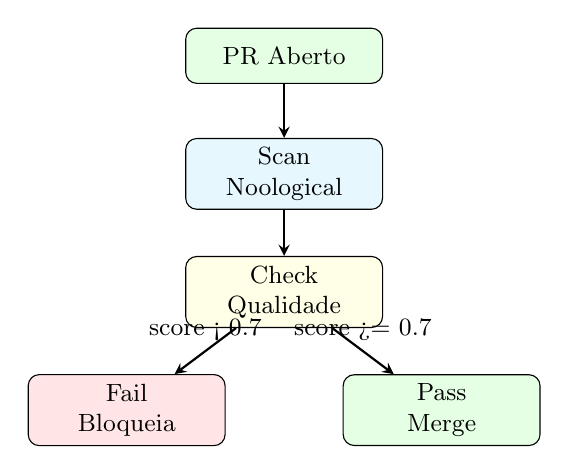
\begin{tikzpicture}[
  node/.style={rectangle, rounded corners, draw, fill=blue!10,
               minimum width=2.5cm, minimum height=0.7cm,
               font=\small, align=center},
  arrow/.style={->, thick, >=stealth}
]
\node[node, fill=green!10] (pr) at (0,2.5) {PR Aberto};
\node[node, fill=cyan!10] (scan) at (0,1.0) {Scan\\Noological};
\node[node, fill=yellow!10] (check) at (0,-0.5) {Check\\Qualidade};
\node[node, fill=red!10] (fail) at (-2,-2) {Fail\\Bloqueia};
\node[node, fill=green!10] (pass) at (2,-2) {Pass\\Merge};

\draw[arrow] (pr) -- (scan);
\draw[arrow] (scan) -- (check);
\draw[arrow] (check) -- node[above, font=\small] {score < 0.7} (fail);
\draw[arrow] (check) -- node[above, font=\small] {score >= 0.7} (pass);
\end{tikzpicture}
\caption{Fluxo de validação automática de PRs com GitHub Actions}
\label{fig:headless-flow}
\end{figure}

O arquivo de workflow do GitHub Actions:

\begin{lstlisting}[style=pythonstyle, caption={Workflow GitHub Actions para
validação automática --- \codigo{.github/workflows/opencode-ci.yml}},
label={lst:github-actions}]
name: OpenCode CI
on:
  pull_request:
    types: [opened, synchronize]

jobs:
  validate:
    runs-on: ubuntu-latest
    steps:
      - uses: actions/checkout@v4

      - name: Setup Node.js
        uses: actions/setup-node@v4
        with:
          node-version: '25'

      - name: Install OpenCode
        run: npm install -g @opencode/cli

      - name: Setup Python
        uses: actions/setup-python@v5
        with:
          python-version: '3.12'

      - name: Start Ollama
        run: |
          docker run -d --name ollama \
            -v $PWD/ollama:/root/.ollama \
            -p 11434:11434 ollama/ollama
          sleep 10
          docker exec ollama ollama pull deepseek-v4-pro

      - name: Run Noological Scan
        run: |
          opencode --headless \
            --command "/scan noological --path $PWD" \
            --output scan-report.json

      - name: Check Quality Gate
        run: |
          SCORE=$(jq -r '.score_completude' scan-report.json)
          if (( $(echo "$SCORE < 0.7" | bc -l) )); then
            echo "Score $SCORE below gate 0.7"
            exit 1
          fi
          echo "Score $SCORE approved"
\end{lstlisting}

\subsection{Exemplo: pipeline de validação de PR}
\label{subsec:pipeline-pr}

Na prática, todo pull request submetido a um repositório configurado com
esse workflow passará pelos seguintes gates:

\begin{enumerate}
\item \destaque{Gate 1 --- Scan Noológico}: verifica se o novo código
      introduz conceitos com cobertura adequada.
\item \destaque{Gate 2 --- Qualidade}: calcula o score de completude.
      Abaixo de 0.7, o PR é bloqueado.
\item \destaque{Gate 3 --- Trust Check} (opcional): avalia o
      comportamento do autor com base no histórico.
\end{enumerate}

\begin{exercicio}
Crie um arquivo \codigo{.github/workflows/opencode-ci.yml} para
um repositório de sua escolha. Adapte o exemplo acima para
incluir também o scanner teleological com um objetivo
personalizado. (\nivelavancado)
\end{exercicio}

% =============================================================================
%  SEÇÃO 9.9: EXERCÍCIOS PRÁTICOS
%  Níveis: zero ao avançado
% =============================================================================
\section{Exercícios Práticos}
\label{sec:exercicios}
\nivelzero\nivelbasico\nivelintermediario\nivelavancado

\paragraph{Praticar é aprender.} Esta seção reúne exercícios de todos os
níveis. Cada exercício inclui um enunciado claro, a saída esperada e uma
dica. Tente resolver sem olhar a dica primeiro.

\subsection{Nível Básico (\nivelbasico)}
\label{subsec:ex-basico}

\begin{exercicio}
Instale o \opencodeeco{} em uma máquina virtual limpa (pode ser um
container Docker). Execute \codigo{opencode doctor} e salve a saída
em \codigo{instalacao.txt}. A saída deve conter a linha
\codigo{Status: OPERACIONAL}.
(\nivelzero)

\destaque{Dica:} Use \texttt{docker run -it ubuntu:24.04} como
ambiente limpo. Instale Node.js, Python e Ollama antes do OpenCode.
\end{exercicio}

\begin{exercicio}
Execute \codigo{/evolve} e observe as cinco etapas do ciclo
evolutivo. Identifique qual etapa consumiu mais tempo. Salve o
relatório gerado em \codigo{evolution/R1/report.json}.
(\nivelzero)

\destaque{Dica:} O relatório contém um campo \codigo{timing} com a
duração de cada etapa. Use \codigo{jq '.timing' report.json} para
extraí-lo.
\end{exercicio}

\begin{exercicio}
Carregue a skill \codigo{research/academic-search} com
\codigo{@skill research/academic-search} e pesquise por
\codigo{machine learning in education}. Liste os três primeiros
resultados. (\nivelbasico)

\destaque{Dica:} Se a skill não estiver disponível, use
\codigo{/skills list} para confirmar o nome exato. O comando é
case-insensitive.
\end{exercicio}

\subsection{Nível Intermediário (\nivelintermediario)}
\label{subsec:ex-intermediario}

\begin{exercicio}
Crie uma skill personalizada que leia um arquivo JSON de
configuração e valide se todos os campos obrigatórios estão
presentes. A skill deve retornar \codigo{valido: true} ou uma lista
de campos ausentes. (\nivelintermediario)

\destaque{Dica:} Use o modelo da Seção~9.3 como base. Defina os
campos obrigatórios em uma lista Python: \codigo{obrigatorios =
[``nome'', ``versao'', ``dependencias'']}.
\end{exercicio}

\begin{exercicio}
Execute \codigo{/scan noological} em um diretório com pelo menos 10
arquivos Python. Identifique a lacuna de maior relevância e crie um
arquivo \codigo{objetivos.json} para o scanner teleological
endereçá-la. Execute \codigo{/scan teleological} e verifique se o
gap foi reduzido. (\nivelintermediario)

\destaque{Dica:} A lacuna de maior relevância é aquela com o maior
produto \codigo{(1 - cobertura) * relevancia}. O scanner
teleological aceita o parâmetro \codigo{--goal} diretamente sem
arquivo.
\end{exercicio}

\begin{exercicio}
Inicie a produção de um artigo com \codigo{/artigo init}. Escolha
um tema relacionado à sua área de atuação. Execute o pipeline até o
estágio de revisão. Anote o score obtido e as sugestões de melhoria.
(\nivelintermediario)

\destaque{Dica:} Se o pipeline completo for muito lento, use
\codigo{/artigo run --fast} que executa apenas os estágios
essenciais (SEEKER + MASWOS + validação rápida).
\end{exercicio}

\subsection{Nível Avançado (\nivelavancado)}
\label{subsec:ex-avancado}

\begin{exercicio}
Crie um pipeline de CI/CD completo usando GitHub Actions que
execute \codigo{/evolve --full} em todo pull request. O pipeline
deve:
\begin{itemize}
\item Bloquear o PR se o score de completude for inferior a 0.7;
\item Comentar no PR o relatório resumido do scan;
\item Opcionalmente, sugerir melhorias automáticas.
\end{itemize}
(\nivelavancado)

\destaque{Dica:} Use a ação \codigo{actions/github-script} para
comentar no PR. O relatório pode ser extraído com
\codigo{jq '.score\_completude' scan-report.json}.
\end{exercicio}

\begin{exercicio}
Aplique \codigo{/reversa} em um projeto open source de médio porte
(50--200 arquivos Python, como Flask ou FastAPI). Analise o grafo
de dependências gerado. Identifique:
\begin{itemize}
\item O módulo com maior acoplamento;
\item Ciclos de dependência, se houver;
\item Padrões de projeto detectados.
\end{itemize}
(\nivelavancado)

\destaque{Dica:} Projetos muito grandes podem exigir ajuste no
parâmetro \codigo{--depth}. Comece com \codigo{--depth 2} e
aumente gradualmente. O relatório completo fica em
\codigo{reversa/report.json}.
\end{exercicio}

% =============================================================================
%  FECHAMENTO DO CAPÍTULO
% =============================================================================
\section*{Síntese do Capítulo}
\label{sec:sintese}
\addcontentsline{toc}{section}{Síntese do Capítulo}

Este capítulo percorreu o caminho prático do \opencodeeco{}, desde a
instalação até a integração com pipelines de CI/CD. A Tabela~\ref{tab:sintese}
sumariza os comandos essenciais aprendidos.

\begin{table}[htb]
\centering
    \small
\caption{Comandos essenciais do OpenCode Ecosystem}
\label{tab:sintese}
    \resizebox{\textwidth}{!}{
\begin{tabular}{clc}
\toprule
\textbf{Comando} & \textbf{Função} & \textbf{Seção} \\
\midrule
\codigo{opencode doctor} & Verificar instalação & 9.1 \\
\codigo{/plan} & Planejar escrita & 9.2 \\
\codigo{/evolve} & Ciclo evolutivo & 9.2 \\
\codigo{/evolve --full} & Pipeline completo & 9.4 \\
\codigo{@skill <nome>} & Carregar skill & 9.3 \\
\codigo{/scan noological} & Mapear conceitos & 9.4 \\
\codigo{/scan teleological} & Avaliar objetivos & 9.4 \\
\codigo{/artigo} & Produção acadêmica & 9.5 \\
\codigo{/reversa} & Engenharia reversa & 9.6 \\
\codigo{/mcps list} & Gerenciar MCPs & 9.7 \\
\codigo{--headless} & Modo não interativo & 9.8 \\
\bottomrule
\end{tabular}
    }
\end{table}

\paragraph{Dica para continuar praticando:}
\begin{itemize}
\item A melhor maneira de aprender o \opencodeeco{} é usá-lo
      diariamente. Comece com tarefas pequenas e aumente a
      complexidade gradualmente.
\item Consulte o Apêndice~\ref{apend:exercicios} para exercícios
      adicionais organizados por área de interesse.
\item O glossário (Apêndice~\ref{apend:glossario}) contém
      definições rápidas de todos os termos técnicos.
\item A comunidade do \opencodeeco{} mantém exemplos e tutoriais em
      \url{https://github.com/MarceloClaro/OpenCode_Ecosystem}.
\end{itemize}
